\documentclass[12pt]{article} % sets up doc as APA manuscript as opposed to journal, and used natbib and apacite for propper citations because that was the best procedure according to the creator of apa6 see here: http://www.tug.org/pracjourn/2012-1/beitzel/beitzel.pdf
\usepackage[margin=1in,footskip=0.25in]{geometry} %Sets up the 
\usepackage[natbibapa]{apacite} 
%\usepackage{natbib}
\usepackage{parskip}
\setlength{\parskip}{6pt}
% \setlength{\parskip}{0pt}
\usepackage{amsmath} % for math text
\usepackage{graphicx} % for graphs and figures
\usepackage[T1]{fontenc} % changing font to text
\usepackage[utf8]{inputenc} % changing font to text
\usepackage{mathptmx} % changing font to text
\setlength{\parindent}{.5in}
\usepackage{setspace}
\renewcommand\bibsection{\centering\refname\parskip}
\usepackage[mdyy]{datetime}
\usepackage{url} % Package for URLs
\usepackage{tikz}
\AtBeginDocument{\urlstyle{APACsame}} % Makes sure URLs in references are formatted correctly.
\usepackage{tabu}
\usepackage{longtable}
\usepackage{titlesec}
\usepackage{amssymb}
\usepackage{cleveref}
\singlespacing
% \doublespacing

\begin{document}
\pagenumbering{gobble}
 \begin{flushright}
	 Deshawn Sambrano\textbf{\\}
	 Bayesian Modeling\\
	 \today
 \end{flushright}
 
 % Send me a one-page outline of your project. This should contain:
 %
 % a one-paragraph description of the nature of the task or data you will model;
 % a one-paragraph or bullet-pointed description of the similarities and differences with the material discussed in class;
 % a one-paragraph or bullet-pointed description of the generative model, if applicable, and of assumptions not captured in the generative model;
 % a one-paragraph or bullet-pointed outline of the questions that you will try to answer.
 % In case you need inspiration, I am putting some interesting Bayesian papers in Resources/Optional Readings
 
 The goal of my project will be to create a Bayesian model that can model data from a random dot motion task (RDM) as an alternative to the standard Drift-Diffusion model (DDM). I will integrate the work of \cite{Bitzer2014} as well as \cite{Fard2017} who have shown how the standard and extended forms of the DDM can be rederived in a Bayesian framework with important benefits of modeling sensory input. While the model's end project will be able to model these type of data, I will run a simulation of various noise and boundary parameters to evaluate their overall effects see final paragraph for details.
 
 This project will tie directly into to and integrate work that we have done in class. In particular, this will incorporate both the evidence accumulation and the classification/Signal Detection Theory lectures. In the cue combination lecture we learned how to integrate multiple pieces of evidences from a single stimulus over time. This is a crucial feature of the DDM, namely that one accumulates (noisy) evidence for a particular option over time. Secondly, SDT has been successful in discriminating between two options and with in this class when learn how to select optimally given specific noise parameters. 
On classic problem in measuring psychological experiments is determining whether one should use reaction time or accuracy in assessing behavioral data. The reason why the classic DDM model has been so popular in perceptual decision making tasks was because it, unlike SDT, integrated both accuracy and reaction time. As such, I will need to incorporate both lectures to complete this project. 

I will adapt the generative model previously proposed \cite{Bitzer2014} and \cite{Fard2017} into a format more consistent with the structure that we have seen in this course. Specifically, I will have a generative model similar to \cref{fig:GModel}. There are several important features not explicitly stated in the generative model. First, there are only two classes $C = 1$ (dot coherence to the right) or $C = -1$ (to the left), while the stimuli are the actual coherence proportions. Second, there are two different CCSDs, this is because I will examine the effects of both distributions. The uniform distribution provides useful information about how the internal and stimulus noise will independently affect inference while the half Gaussian will be more similar to how most experiments are designed, so I wanted to explore both. Third, the inference of interest is the class of the stimulus (either left or right). Fourth, we will require a hidden variable $\lambda$ by which we set our criterion (for completeness, I will use three different ones high, medium, and low). This mimics the case for SDT when we specified the criterion k for making a decision (optimal would be 0 for log odds, but we could have chosen another criterion value). And fifth and perhaps most importantly, there are two subtleties with the $x's$. First, as is the case with DDM these represent the participants sequential evidence accumulation steps in time of the same stimulus AND on the same trial. This means that we are proposing a situation where we predict multiple stages of cue combination over time even though the participant only provides one response per trial (the same goes for DDMs) and this is resolved by examining the reaction time for the given trial. The time it takes to respond yields critical information about the rate of evidence accumulation for the given stimuli type (in other words the difficulty of discerning class). Second, and again as with the case for DDMs, we will assume that these pieces of evidence are conditionally independent. 

\begin{figure}
	\begin{center}
		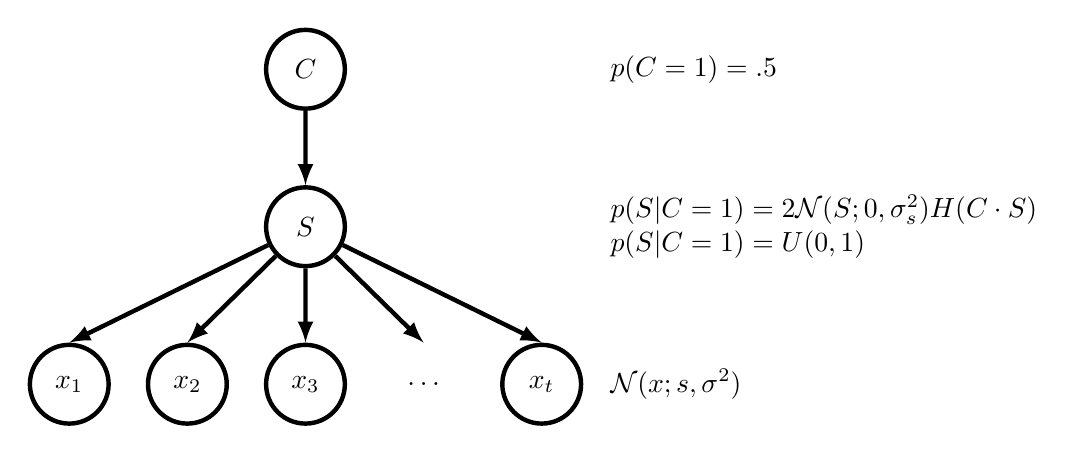
\begin{tikzpicture}[xscale=1.5]
			\tikzstyle{arrow}=[draw, -latex]
			\newcommand\Xmax{5}
			\newcommand\XMid{\Xmax/2}
			\newcommand\Xtext{\Xmax}

			\newcommand\YSpace{2}
			\newcommand\Yclass{1.5}
			\newcommand\YStim{\Yclass-\YSpace}
			\newcommand\Yxs{\YStim-\YSpace}

			% Grid
			% \draw [help lines] (0,-5) grid (7,3);
			 % Class
			\node [draw, circle, minimum width=1cm, ultra thick] at (\XMid,\Yclass) (C) {$C$};
			\node [anchor=west] at (\Xtext, \Yclass) (Cstat) {$p(C = 1) = .5$};

			 % Stimulus
			\node [draw, circle, minimum width=1cm, ultra thick] at (\XMid,\YStim) (S) {$S$};
			\node [anchor=west, align=left] at (\Xtext, \YStim) (Cstat) {$p(S|C = 1) = 2\mathcal{N}(S;0,\sigma_s^2)H(C\cdot S)$\\$p(S|C = 1) = U(0,1)$};

			 % Observations
			\node [draw, circle, minimum width=1cm, ultra thick] at (.5,\Yxs) (x1) {$x_1$};
			\node [draw, circle, minimum width=1cm, ultra thick] at (1.5,\Yxs) (x2) {$x_2$};
			\node [draw, circle, minimum width=1cm, ultra thick] at (2.5,\Yxs) (x3) {$x_3$};
			\node [draw, circle, minimum width=1cm, ultra thick, white] at (3.5,\Yxs) (dots) {\textcolor{black}{$\ldots$}};
			\node [draw, circle, minimum width=1cm, ultra thick] at (4.5,\Yxs) (xt) {$x_t$};
			\node [anchor=west] at (\Xtext, \Yxs) (Cstat) {$\mathcal{N}(x;s,\sigma^2)$};
  
			 % Path Arrows 
			\path [arrow, ultra thick] (C) -- (S);
 
			\path [arrow, ultra thick] (S) -- (x1.north);
			\path [arrow, ultra thick] (S) -- (x2.north);
			\path [arrow, ultra thick] (S) -- (x3.north);
			\path [arrow, ultra thick] (S) -- (dots.north);
			\path [arrow, ultra thick] (S) -- (xt.north);
 
		\end{tikzpicture}
	\end{center}
\caption{\label{fig:GModel}Generative Model.}
\end{figure} 
 The question I intend to answer with this project is three-fold: 1) what role do external (stimulus) and internal noise play in the amount of time it would take for a Bayesian observer to accumulate enough evidence to reach the thresholds ($\lambda$), 2) explore how the various levels of requested accuracy will influence time to accumulate sufficient evidence, and 3) evaluate the role of both noise and $\lambda$ on predicted number of correct and incorrect (and non response) responses given a an experimenter implemented time limit. This is mostly experimentally relevant because most of these designs have a time limit, such that a Bayesian observer with enough noise might still be able to accumulate enough evidence, but sufficiently quick enough to make a response in time.  
 
 %\newpage
 
 % \begin{center}
% 	 \textbf{Methods}
%  \end{center}
%  \textbf{Participants}
%
%
% Preliminary analyses were conducted on 45 individuals (66\% Females, 33\% Caucasian, \emph{$M_{age}$} = 24.8, \emph{$SD_{age}$} = 7.7). I anticipate collecting 30 more participants (for a total of 75) by the end of the semester; however, this estimate is conditional on how soon the IRB protocol is approved.
%
% \noindent\textbf{Analytic Plan}
%
% \textbf{Decision Processing.}\hspace{2mm} Two scales were created for this study and each will be addressed separately. The first scale that was created was a decision making style scale. A previous scale has already been created on this topic, the General Decision Making Style scale \citep[GDMS; See Appendix A; ][]{Scott1995} but this scale had several limitations. First, the original scale was a 25-item scale to created five factors, one per decision style proposed by the authors. However, decision making is often characterized by two styles--analytic and intuitive--which manifest from two systems of thought described as dual system theory \citep[e.g., ][see \citeauthor{Phelps2014}, \citeyear{Phelps2014} for review]{ Kahneman2011}. Although the dual system theory of decision making debated, researchers often need a quick assessment of a persons decision style (e.g., as a manipulation check). Yet no simple measures (under 10 items) have been developed. The aim of this scale was to reduce the number of items of the GDMS scale to assess the extent to which people use analytic versus intuitive decision styles.
%
% Item Response Theory (IRT) will be used to evaluate the psychometric properties of this scale because of the copious advantages of IRT of classical test theory: it provides item based parameter-free sample estimates and sample-free parameter estimates,  provides better true score estimates, and allows each item to function independently which allows poorly functioning items to be identified within a scale that might otherwise be classified as a poor scale \citep{Reise2003}. Because limited information about the scales psychometric properties have examined, the Nominal Response Model \citep[NRM; ][]{Bock1972} within IRT will be used. The NRM is provides a model to test unordered categories of responses \citep{deAyala1999}. The NRM serves as the exploratory (least constrained) form of the divide-by-total \citep{Thissen1986} IRT models \citep{Preston2014}. As such, the NRM response model is most equip to handle scales that may have a one or several items with poorly functioning categories.
%
%
% \textbf{\emph{Assumption Assessment}.}\hspace{2mm} Although the original scale was multidimensional, the reduced version was designed to be unidimensional, in part to fit the assumption of IRT. Specifically, the analytic and intuitive factors of the original scale will be used. Dual system theories propose that intuitive and analytic decision styles are combative and working in opposition. Aligned with that proposal intuitive items will be reverse coded prior to analyses. This structural was used in order to create a single dimension from intuitive (low of latent trait) to analytical (high on the latent trait). \cite{Reise2014} review a series of studies that demonstrate the robustness of violations of unidimensionality for IRT models. In fact, \citeauthor{Reise2014} suggests that data only need to be ``unidimensional enough.'' For the present scale, data will be analyzed with polychroic correlations through the Comprehensive Exploratory Factor Analysis \citep[CEFA, ][]{Browne1998} to assess for unidimensionality. Specifically, the eigenvalues will be evaluated. If the the first eigenvalue accounts for more than 60\% of the variance in the first factor, the data are assumed to be ``unidimensional enough'' for IRT. If data are not unidimensional, one of two actions will be taken. If there are only a few items the violate unidimensionality and there is sufficient theoretical justification to remove them, they will be eliminated. If there are a substantial number of items that would create an additional factor, the test will be split into testlets. One testlet will serve as the intuitive decision style and the other will serve as the analytic decision style.
%
%
% Crucially for appropriate modelling of the data, the latent trait (use of an analytic decision style) is assumed to be continous and monotonic for the present scale. Finally, for appropriate interpretation and generalization of the parameter estimates the model must fit the data. I anticipate that initial models will not fit the data because they will serve as explorations into the psychometric properties of the scale and because I do not anticipate to obtain a large enough sample size to effectively estimate the parameters. However, the parameter estimates will survey as guidelines for survey development. Specifically, items that are poorly functioning (i.e., provide little to no information), have poorly functioning categories (assessed via a and b parameter estimates and standard errors as well as category boundary discrimination (CBD) parameters), or are redundant (provided the same or less information about the latent construct at a given location compared to other items) will be either deleted entirely or will have their categories adjusted. These alterations will help to ensure model fit and maximize the usability of parameter estimates and of the scale constructed.
%
%
% \textbf{Information Processing.}\hspace{2mm} A person's decision making style is highly related to their processing style. Information processing style has been previously measure using the Cognitive Reflection Task \citep[CRT, ][]{Frederick2005}. The scale utilizes series of riddles to assess processing style. Unfortunately, the riddles have been utilized for several years, and their reliability may be reduced since people already know the answers. As such, I have created three new questions that mimic the structure of CRT to allow for a rejuvenated measure of processing style. These items follow a similar structure and probe the same construct as the the original CRT (see Appendix B).
%
%
% For reasons explicated above, I will use IRT to assess the psychometric properties of the adjusted CRT. However, due to the nature of the response format NRM will not be used. Responses will are either open ended or multiple with a designated order. Specifically, there is one correct answer and all others are assumed to be equally wrong. As such the 2 parameter logistic (2PL) IRT model will be used for these data. \citep{Reise2003} suggest that the 2PL fits most data of this structure. However, the 2PL, 1PL, and 3PL will compared to ensure the best model fit.
%
%
% \textbf{\emph{Assumption Assessment}.}\hspace{2mm} The original CRT was designed as a unidimensional construct. Since the newly created items were only extension questions designed to assess the same construct, I expect that the data will reveal a unidimensional construct. The same CEFA procedures described above will be used to assess unidimensionality for as above will be used and will include both the old CRT and the new created questions. If data are not unidimensional, items will be removed until a single construct (use of analytic processing style) is measured. The new scale will yield to the previous data to determine whether it met the assumptions of IRT. The initial assessment of the CRT provided evidence that the latent trait is continous and monotonic such that as you increase on the laten trait you increase on the proportion responded correctly. The model generalizability and interpretability hinders on whether the model fits the data or not. This is why the 1PL, 2PL, and 3PL will be compared to identify to best model fit.
%
%
% % This alignes well with previous
% % Continuous latent trait
% % monotonic relationship between latent trait and thing
% % model fits the data.
%
%
% \textbf{Validity.}\hspace{2mm} In addition to collecting information on participants decision and processing style, their need for cognition \citep[NFC; ][]{Cacioppo1984} was also assessed. The scale measures individual differences in the desire for cognitive stimulation and challenge. This is an ideal scale for this research because NFC should be highly related to analytic decisions and processing styles. Since the purpose of this study will be to evaluate the psychometric properties of the decision and processing styles scales, the psychometric properties of NFC will not be evaluated. Furthermore, this study will rely upon previous work done on the NFC \citep[e.g., ][among others]{Cacioppo1984}. Previous research hase demonstrated the properties of the NFC through sum scores and that will be used for this study as well. Validity of the two proposed scales will be assessed in the following ways: (a) the correlation between the decision making style scale score ($\theta$) and the information processing style $\theta$ and (b) the magnitude of relationship between each of the scales the the NFC sum scores. To demonstrate maximal validity, decision and processing style $\theta$'s should be more strongly related to each other than to NFC.
%
%
% % An intuitive decision is characterized by fast, automatic and intuitive choices, while analytic decisions are characterized by slow, deliberative and analytic decisions. Each decision style is closely tied to of the two systems of thinking \citep{Kahneman2011}. This distinction of decision styles provides useful predictive insights into the choices a person will make. Further, given the ubiquitous nature of choices, some with severe consequences for ourselves and others (e.g., careers choices and jury decisions), exploring what leads to analytic vs. intuitive is imperative, and this scale can assist researchers in this process.
%
%
% % There have been previous scales designed to assess decision styles \citep{Nygren2002, Scott1995}, but these studies have all used classical test theory. One issue with these scales is they assess decision making styles as a multi-dimensional attribute that is not purvey to experimental designs simply trying to differentiate between intuitive and analytic styles. Further, these  questions are based on general style, without reference to the current context. Appendix A lists the questions from \cite{Scott1995} and indicates the items that I will use for my scale. This scale is used because it has been validated by several studies and used fairly regularly. As such it serves as a satisfactory basis for the development of a new scale.
%
%
% % \citeauthor{deBruin2007}'s \citeyearpar{deBruin2007} decision outcome inventory (DOI) measures participants' satisfaction with the outcome of their decisions. This measure has been shown relate to \citeauthor{Scott1995}'s \citeyearpar{Scott1995} scale and was use a validation measure in previous studies \citep{deBruin2007}.



\bibnewpage
\bibliographystyle{apacite}
\raggedright
\doublespacing
%\setlength\bibsep{\baselineskip}
\setlength\bibhang{.5in}
  \bibliography{mybib}
  

  \newpage
%  \begin{center}
  \appendix
  \setlength{\parskip}{0pt}
  \titlespacing*{\section}{0pt}{0pt}{-15pt}
  \section*{\centering\normalsize\textnormal{Appendix A\\ 25-item General Decision Making Style Scale}}
  \label{appendix:GDMS}
  \singlespacing
  \newcolumntype{L}{>{\raggedright\hangindent=2em}X[1]}
\setlength{\extrarowheight}{3pt}
\begin{tabu} to \linewidth{LL}
\hline
\multicolumn{2}{p{\linewidth}}{\textbf{Instructions}: Please indicate the extent to which you each sentence captures how you are \newline\textbf{CURRENTLY} make decisions.}\vspace{6pt}\\
\hline
I double-check my information sources to be sure I have the right facts before making decisions. & I make decisions in a logical and systematic way.\\
My decision making requires careful thought. & When making a decision, I consider various options in terms of a specific goal.  \\
When making decisions, I rely up my instincts. & When I make decisions, I tend to rely on my intuition. \\
I generally make decisions that feel right to me. & When I make a decision, it is more important for me to feel the decision is right than to have a rational reason for it. \\
When I make a decision, I trust my inner feelings and reactions. & I often need the assistance of other people when making important decisions. \\
I rarely make important decisions without consulting other people.$^a$ & If I have the support of others, it is easier for me to make important decisions.$^a$ \\
I use the advice of other people in making my important decisions.$^a$ & I like to have someone to steer me in the right direction when I am faced with important decisions.$^a$ \\
I avoid making important decisions until the pressure is on. & I postpone decisions making whenever possible.$^a$ \\
I often procrastinate when it comes to making important decisions.$^a$ & I generally make important decisions at the last minute. \\
I put off making many decisions because thinking about them makes me uneasy.$^a$ & I generally make snap decisions. \\
I often make decisions on the spur of the moment. & I make quick decisions. \\
I often make impulsive decisions. & When making decisions, I do what seems natural at the moment. \\
I explore all of my options before making a decision.\vspace{6pt}\\
\hline
\multicolumn{2}{p{\linewidth}}{\emph{Note}: $^a$ indicates elements that are only in the 25-item version. All other items will be assessed in both scales. All items will be assess on a 5-point Likert-type scale (1 = \emph{Strongly disagree} to 5 = \emph{Strongly agree}, as was used in the original scale).}
\end{tabu}
\doublespace



  \newpage
  \section*{\centering\normalsize\textnormal{Appendix B\\ Cognitive Reflection Task with new Sample Items}}
  \singlespacing
\setlength{\extrarowheight}{6pt}
\begin{tabu} to \linewidth{X[.2]>{\raggedright\hangindent=2em}X}
Old CRT & A bat and a ball cost \$1.10 in total. The bat costs \$1.00 more than the ball. How much does the ball cost? \_\_\_\_ cents.  \textbf{Answer Format}: Open response\\
Old CRT & If it takes 5 machines 5 minutes to make 5 widgets, how long would it take 100 machines to make 100 widgets? \_\_\_\_ minutes.  \textbf{Answer Format}: Open response\\
Old CRT & In a lake, there is a patch of lily pads. Every day, the patch doubles in size. If it takes 48 days for the patch to cover the entire lake, how long would it take for the patch to cover half of the lake? \_\_\_\_ days.  \textbf{Answer Format}: Open response\\
CRT 2.0 & If you’re running a race and you pass the person in second place, what place are you in? \textbf{Answer Choices}: \textit{First, Second, Third}\\
CRT 2.0 & A farmer had 15 sheep and all but 8 died. How many are left? \_\_\_\_ sheep. \textbf{Answer Format}: Open response\\
CRT 2.0 & Emily’s father has three daughters. The first two are named April and May. What is the third daughter’s name? \_\_\_\_ \textbf{Answer Format}: Open response\\
CRT 2.0 & How many cubic feet of dirt are there in a hole that is 3’ deep x 3’ wide x 3’ long? \_\_\_\_ cubic feet of dirt. \textbf{Answer Format}: Open response\\
New Sample & If one car take 100 minutes to travel 100 miles, how fast is the car traveling? \_\_\_\_ $\frac{miles}{hour}$ \textbf{Answer Format}: Open response\\
New Sample & Alice is looking at Bob, and Bob is looking at Charlie. Alice is married and Charlie is not married. Is a married person looking at an unmarried person? \textbf{Answer Choices}: \textit{Yes, no, cannot be determined}\\
New Sample & A drawer has 10 black socks and 10 white socks. With your eyes closed you pull 3 socks from a drawer. Are you holding a pair of socks? \textbf{Answer Choices}: \textit{Yes, no, cannot be determined}
\end{tabu}
\doublespace

  \newpage
  \section*{\centering\normalsize\textnormal{Appendix C\\ CEFA Output to Assess for Unidimensionality}}
  
  
  \newpage
  \section*{\centering\normalsize\textnormal{Appendix D\\ IRT Output Demonstrating I know the appropriate code to run (and that I do not have the sample size to estimate these parameters)}}


\end{document}